\chapter{Mængder og sæt}
Et sæt er en endelig eller uendelig mængde af objekter hvor rækkefølgen ingen vigtighed har og mulitiplicitet generelt ignoreres (modsat lister og multisæt). Medlemmer af en mængde kaldes for elementer og notationen $a\in A$ viser at $a$ er et element i sættet $A$. 

Store bogstaver ($A$, $B$, $X$, $Y$, osv) betegner mængder, mens små bogstaver ($a$, $b$, $x$, $y$, osv.) betegner elementer. Rækkefølgen af elementerne i et sæt er ligegyldig, således er $X=\left\{ 1,2,3\right\}$ og $Y=\left\{ 2,3,1\right\}$ lige med hinanden. 
Et sæt som intet indeholder kaldes tomt (\textbf{eng}: \textit{empty}, \textit{null} eller \textit{void}) og denoteres $\emptyset$, hvor $\emptyset = \{\}$.
\section{Prædefinerede sæt}
\textbf{Mængden af alle heltal} har bogstavet \textbf{Z} (eller $\mathbb{Z}$), hvor $\mathbb{Z}=\{\ldots, -2, -1, 0, 1, 2, \ldots\}$ (når udeladelsesprikker benyttes til sidst eller først, antyder det at den fortsætter \emph{uendeligt} i den retning).\\
\textbf{Mængden af alle positive tal (naturlige tal)} har bogstavet \textbf{N} (eller $\mathbb{N}$), hvor $\mathbb{N}=\{1,2,3,\ldots\}$. Således er et naturligt tal et positivt heltal.\\
\textbf{Mængden af alle reelle tal} har bogstavet \textbf{R} (eller $\mathbb{R}$), hvor $\mathbb{R}$ kan beskrive ethvert tal, mens $R^+$ beskriver ethvert positivt, og så videre.\\
\textbf{Mængden af rationelle tal} har bostavet \textbf{Q} (eller $\mathbb{Q}$) og er et reelt tal som kan udtrykkes som en kvotient af to heltal\[\frac{m}{n}\quad, \text{hvor } m,n\in \mathbb{Z}\]hvor $n$ naturligvis ikke må være nul ($n\neq 0$).\\
\textbf{Mængden af irrationelle tal} har ikke officielt noget bogstav (men \textbf{I} eller $\mathbb{I}$ kan benyttes) er ethvert reelt tal som ikke kan beskrives som en kvotient. Et sådan tal har (uendelige) ikke-periodiske decimaler. Eksempler på disse er $\sqrt{2}$, $\sqrt{3}$, $\sqrt[3]{2}$, $\pi$ og $e$.
\subsection{Kardinalitet \texorpdfstring{-- $|A|$}{|A|}}
Kardinaliteten (eller kardinaltallet) for en mængde $S$ er givet ved $|S|$, og betegner antallet af elementer i $S$. Det er her vigtigt at huske at en mængde også kun fungerer som ét element. Ved $A=\{1,2,\{3,4\},5\}$ vil det for $A$'s kardinaltal gælde at $|A|=4$.
\subsubsection{Eksempel}
Lad $D=\{n\in\mathbb{N}:n\leq 9\}, E=\{x\in\mathbb{Q}:x\leq9\}, H=\{x\in\mathbb{R}:x^2-2=0\}$ og $J=\{x\in\mathbb{Q}:x^2-2=0\}$.
\begin{enumerate}
    \item \textit{Beskriv mængden $D$ ved at opskrive dens elementer.}\\ $D=\{1,2,3,4,5,6,7,8,9\}$.
    \item \textit{Giv et eksempel på tre elementer som tilhører $E$ men ikke tilhører $D$.}\\$-2$, $8.9$, $1.5$.
    \item \textit{Beskriv mængden $H$ ved at opskrive dens elementer.}\\ $H=\{-\sqrt{2}, \sqrt{2}\}$.
    \item \textit{Beskriv sættet $J$ på en anden måde.}\\Ligningen har ingen løsninger indenfor de rationelle, hvorfor $J=\emptyset$.
    \item \textit{Bestem kardinaliteten for hvert sæt $D, H$ og $J$.}\\ $|D|=9$, $|H|=2$ og $|J|=0$.
\end{enumerate}
\section{Delmængder \texorpdfstring{-- $\subset$}{}}
Et sæt $A$ er en delmængde af $B$ hvis ethvert element af $A$ også tilhører $B$. Hvis $A$ er en delmængde af $B$, så skriver man $A\subseteq B$, hvorved $B$ er en supermængde af $A$: $A\supseteq B$. Således gælder det at $\mathbb{N}\subseteq \mathbb{Z}$, $\mathbb{Q}\subseteq \mathbb{R}$ og $\mathbb{Q}\subseteq \mathbb{R}$. Da $\mathbb{Q}\subseteq \mathbb{R}$ og $\mathbb{R}\subseteq \mathbb{C}$, følger det at $\mathbb{Q}\subseteq \mathbb{C}$. Det gælder desuden at hver mængde er dets eget delmængde. Det gælder dog at $\mathbb{Z}\subsetneq \mathbb{N}$.
\section{Mængdeoperatorer}

\subsection{Foreningsmængde \texorpdfstring{-- $\cup$}{}}
Foreningen af to mængder $A$ og $B$ skrives $A\cup B$ (\textbf{eng}: \textit{union}; \textbf{latex}: \texttt{cup}), og er det sæt af elementer som tilhører $A$ eller $B$; altså \[A\cup B = \left\{ x:x\in A \lor x\in B\right\}\]
hvor \textit{eller} ($\lor$) betyder at et element i $A\cup B$ både kan tilhøre $A$ og $B$. Således vil $x$ være i $A\cup B$ hvis
\begin{enumerate}
    \item $x$ er i $A$
    \item $x$ er i $B$
    \item $x$ er i både $A$ og $B$
\end{enumerate}
Et Venn-diagram kan bruges til at illustrere dette på. Se figur \ref{fig:foreningvenn}.
\begin{figure}[H]
    \centering
    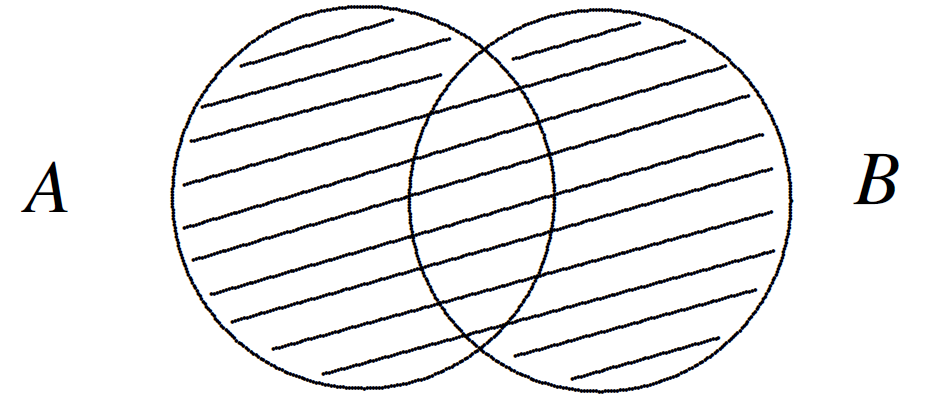
\includegraphics[width=0.4\textwidth]{billeder/Acrobat_h4xoc29CTB.png}
    \caption{Venn-diagram, hvor det tonede område betegner $A\cup B$}
    \label{fig:foreningvenn}
\end{figure}
\subsection{Fællesmængde \texorpdfstring{-- $\cap$}{}}
Fællesmængden af to mængder $A$ og $B$ skrives $A\cup B$ (\textbf{eng}: \textit{intersection}; \textbf{latex}: \texttt{cap}), og er det sæt af elementer som både tilhører $A$ og $B$; altså \[A\cap B=\{ x:x\in A \land x\in B\}\]
Et Venn-diagram kan bruges til at illustrere dette på. Se figur \ref{fig:fellesvenn}.
\begin{figure}[H]
    \centering
    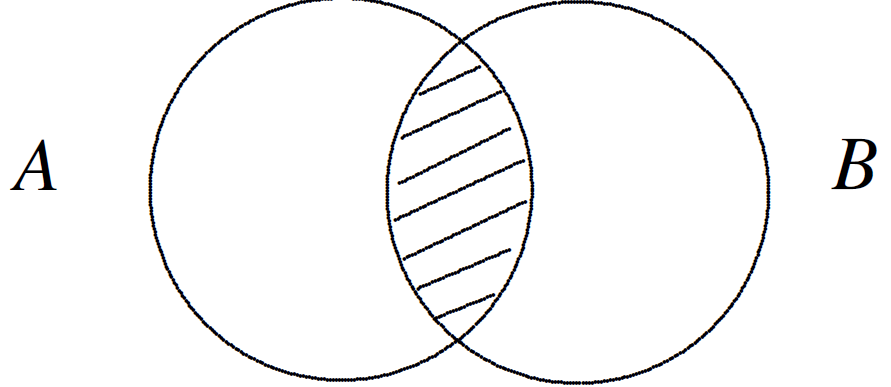
\includegraphics[width=0.4\textwidth]{billeder/Acrobat_bHAl8Wuekv.png}
    \caption{Venn-diagram, hvor det tonede område betegner $A\cap B$}
    \label{fig:fellesvenn}
\end{figure}
\subsubsection{Disjunkt}
Hvis to mængder ikke har nogle elementer tilfælles siges de at være disjunkt, altså adskilte. For to disjunkte mængder gælder det at \[A\cap B = \emptyset\]
Sammenhængen mellem foreningsmængde og fællesmængde er\[A\cap B\subseteq A\cup B\]
\subsection{Mængdedifferens og relativ komplementærmængde \texorpdfstring{$-$ eller $\setminus$}{}}
Differensen $A-B$ af to mængder $A$ og $B$ (også skrevet $A\setminus B$) er defineret som\[ A-B=\{x:x\in A\,\land x\notin B\}\]Et Venn-diagram kan bruges til at illustrere dette på. Se figur \ref{fig:differensvenn}.
\begin{figure}[H]
    \centering
    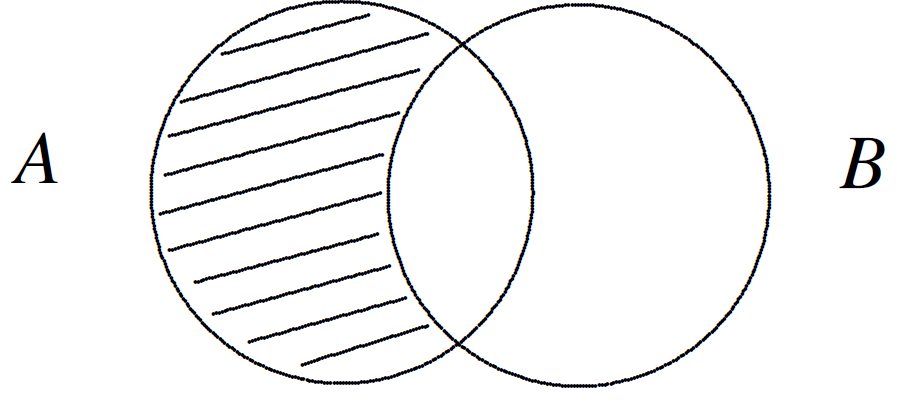
\includegraphics[width=0.4\textwidth]{billeder/Acrobat_mR0KSCJDtQ.png}
    \caption{Venn-diagram, hvor det tonede område betegner $A-B$}
    \label{fig:differensvenn}
\end{figure}
\textit{Mængdedifferensen kaldes også for \textbf{den relative komplementærmængde}. (læs mere om komplementærmængder i nedenunder)}
\subsection{Komplementærmængde\texorpdfstring{ -- $\overline{A}$}{}}
Komplementærmængden $\overline{A}$ af $A$ er mængdedifferensen af universalmængden $U$ og $A$; altså\[\overline{A}=\{x:x\in U \land x\notin A\}\]Et Venn-diagram kan bruges til at illustrere dette på. Se figur \ref{fig:complementvenn}.
\begin{figure}[H]
    \centering
    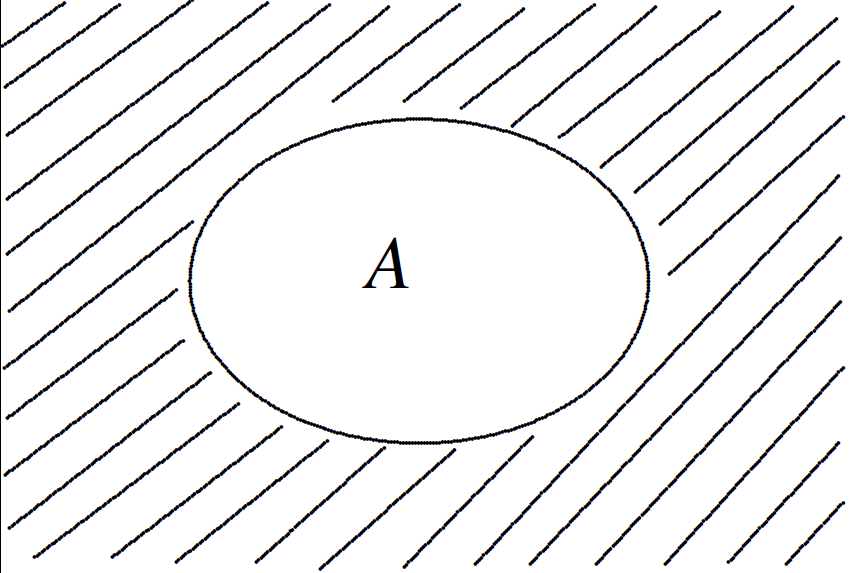
\includegraphics[width=0.4\textwidth]{billeder/Acrobat_p0XoSIqOY7.png}
    \caption{Venn-diagram, hvor det tonede område betegner $\overline{A}$}
    \label{fig:complementvenn}
\end{figure}
\subsection{Mange mængder}
Ønsker man at behandle flere mængder bør man indeksere disse. Har man $n$ sæt, $A_1, A_2, \ldots, A_n$, så vil disses \textbf{foreningsmængde} være $A_1\cup A_2\cup \ldots \cup A_n$, eller bare $\bigcup_{i=1}^n A_i$ og er defineret som enhver værdi som befinder sig i sættene\[\bigcup_{i=1}^n A_i = \{x:x\in A_i \text{ for en } i, 1\leq i\leq n\}\]
\textbf{Fællesmængden} for disse er udtrykt ved $A_1\cap A_2\cap\ldots\cap A_n$ eller $\bigcap_{i=1}^n A_i$ og er defineret som enhver værdi som er i alle sættene\[\bigcap_{i=1}^n A_i=\{x:x\in A_i \text{ for alle } i, 1\leq i\leq n\}\]
\section{Partition og deling}
Hvis to mængders fællesmængde er tom, da siges de at være disjunkte. Hvis en samling\footnote{En samling er en mængde som består af mængder.} $\mathcal{S}$ er en delmængde af mængden $A$ er den \textbf{parvist disjunkt} hvis et vilkårligt delmængde-par som tilhører $\mathcal{S}$ er disjunkt.\par\textbf{Eksempel.} Lad $A=\{1,2,\ldots,7\}$, $B=\{1,6\}$, $C=\{2,5\}$, $D=\{4,7\}$ og $S=\{B,C,D\}$. Herved er $S$ en parvis disjunkt samling af delmængder af $A$ da\[B\cap C=B\cap D=C\cap D=\emptyset\]\par
En \textbf{partition} af en mængde $A$ er en samling $\mathcal{S}$ af ikke-tomme delmængder af $A$ således at hvert element af $A$ tilhører præcist én delmængde i $\mathcal{S}$. Altså vil en partition af $A$ være den samling $\mathcal{S}$ af delmængder af $A$ som tilfredsstiller
\begin{enumerate}
    \item $X\neq\emptyset$ for hvert sæt $X\in\mathcal{S}$
    \item for hver par af mængder $X,Y\in\mathcal{S}$, vil enten $X=Y$ eller $X\cap Y=\emptyset$
    \item $\bigcup_{X\in\mathcal{S}}X=A$
\end{enumerate}\par\textbf{Eksempel.} Mængden af reelle tal $\mathbb{R}$ kan partitioneres/deles op i tre mængder: Mængden af alle positive, reelle tal ($\mathbb{R}^+$); Mængden af alle negative, reelle tal ($\mathbb{R}^-$); Mængden som består af nul ($\{0\}$). Således at $S_\mathbb{R}=\{R^-, \{0\}, R^+\}$.
\section{Jan Philip Solovejs forelæg 02-09}
Der er forskel på tal. Der er nemme tal (naturlige tal; $\mathbb{N}=\lbrace0,1,2,\ldots\rbrace$), men også algebraiske tal og ikke-matematiske tal (som ikke kan bestemmes ved matematiske beregninger, men er afhængige af målinger). De hele tal ($\mathbb{Z}=\lbrace\ldots,-1,0,1,\ldots\rbrace$), de rationelle tal ($\mathbb{Q}=\lbrace\frac{p}{q}:p\in \mathbb{Z},q\in\mathbb{N}\rbrace$), og de irrationelle tal.

\begin{proof}{Hvis $a$ er ulige: $a=2n-1$.}
\begin{lemma}Hvis $a\in\mathbb{N}$ og $a$ er ulige, da er $a^2$ ulige.\end{lemma}
Vi ved at $a^2=(2n-1)^2=4n^2+1-4n=2(2n^2-2n)+1$, altså vil produktet af ulige tal give et ulige tal. Det samme gælder for primtalsfaktorisering, hvor alle lige tal faktoriseres med 2.
\end{proof}

\begin{proof}{$\sqrt{2}\notin\mathbb{Q}$}
Antag at $\sqrt{2}=\frac{n}{m}\implies\sqrt{2m}=n\implies2m^2?n^2\implies n\text{ er lige}$, hvor $\frac{n}{m}$ er uforkortelige. Altså $n=2p\text{ hvis }p\in\mathbb{N}$.\\$2m^2=n^2=(2p)^2=4p^2\implies m^2=2p^2$, hvorved både $m$ og $n$ er lige, hvorfor $\sqrt{2}$ må være et irrationelt tal.
\end{proof}
Reelle tal $\mathbb{R}$ er tal, der kan tilnærmes med rationelle tal. Notationen for mængder er ved åbent interval $$]a,b[=(a,b)=\lbrace x\in\mathbb{R}|a<x<b\rbrace$$mens lukkede er $$[a,b]=\lbrace x\in\mathbb{R}|a\leq x\leq b\rbrace$$Den numeriske værdi er talværdien, eller den absolutte værdi $|a|=\begin{cases}
    \,\,\,\,\,a, \,\, a\geq0\\
    -a, \,\,a<0
  \end{cases}$
  
Lige meget hvilket reelt tal man vælger, vil der altid være et naturligt tal som er større. <- Arkimedes princip.

\begin{proof}{$a,b\in\mathbb{R}$ og $a<b$ da vil intervallet $(a,b)$ indeholde både rationelle og irrationelle tal, lige meget hvor småt, altså at $(a,b)\cap \mathbb{Q}\neq \emptyset$}, mens $(a,b)\cap(\mathbb{R}\setminus\mathbb{Q}\neq\emptyset$

\end{proof}
\textbf{Fuldstændighedsegenskaben:} Hvis $A\subseteq\mathbb{R}$ og $A\subseteq(-\infty,b]$ $b\in\mathbb{R}$. Enhver mængde $A$ som er indeholdt i $(-\infty,b)$ fra et eller andet $b$ har en mindste øvre grænse, altså supremum, $\text{sup}A$. I $\text{sup}(-2,3)=3$ og $\text{sup}(-2,3]=3$ <- her et ekstremum.

En metode til at finde rødder i polynomier er ved at bryge polynomiers division: Man kan dividere roden ud, hvis man kender en anden rod. Eksempel: $\frac{x^2+5x+7}{x+2}$

\subsection{Komplekse tal}Vi indfører $\sqrt{-1}=i$ løser $x^2+1=0\implies x=\pm i$. Definition: $i^2=-1$. Når man ganger to komplekse tal foregår det ved $(2+3i)(1+i)=2(1+i)+3i(1+i)=2+2i+3i+3i^2=2+5i-3=-1+5i$. Mængden af komplekse tal er givet ved \begin{equation}
    \mathbb{C}=\{a+ib|a,b\in\mathbb{R}\}
\end{equation}